\documentclass[sigconf]{acmart}

\usepackage{booktabs} % For formal tables
\usepackage{subfig}
\usepackage{cite}

\begin{document}
\title{Demo Paper: Demonstrating Hybrid Provenance Queries from Script Runs}


%\author{Ben Trovato}
%\orcid{1234-5678-9012}
%\affiliation{%
%  \institution{Institute for Clarity in Documentation}
%  \streetaddress{P.O. Box 1212}
%  \city{Dublin} 
%  \state{Ohio} 
%  \postcode{43017-6221}
%}
%\email{trovato@corporation.com}

%\author{G.K.M. Tobin}
%\affiliation{%
%  \institution{Institute for Clarity in Documentation}
%  \streetaddress{P.O. Box 1212}
% \city{Dublin} 
%  \state{Ohio} 
%  \postcode{43017-6221}
%}
%\email{webmaster@marysville-ohio.com}

%\author{Lars Th{\o}rv{\"a}ld}
%\affiliation{%
%  \institution{The Th{\o}rv{\"a}ld Group}
%  \streetaddress{1 Th{\o}rv{\"a}ld Circle}
%  \city{Hekla} 
%  \country{Iceland}}
%\email{larst@affiliation.org}


% The default list of authors is too long for headers}
%\renewcommand{\shortauthors}{B. Trovato et al.}


\begin{abstract}
In this demo, we demonstrate prospective and retrospective provenances collected by YesWorkflow (YW) and DataONE RunManagers (R client and MATLAB client). For a workflow project, we have multiple provenance graphs consisting of a graph of prospective provenance, a graph of hybrid provenance, a graph of retrospective multi-run provenance. From our demonstration, we find that the demonstrated provenance capabilities can benefit earth researchers to understand the processing history of a derived products and verify them. 
\end{abstract}


\keywords{prospective provenance, hybrid provenance, retrospective provenance, hybrid provenance query, retrospective provenance query}

\maketitle

\section{Introduction}

Provenance from scripts and runs of scripts plays an important role in software debugging, testing, reliability and sharing. Such provenance traces consist of events that the user is interested in. A considerable amount of research has been done on investigating methods of harvesting provenance information from scripts and runs of scripts, ranging from conventional approaches, e.g. research compendium (folder layouts) and logging to recent provenance tools, e.g., YesWorkflow (YW) [ref], noWorkflow (NW) [ref], RDataTracker [ref], Reprozip [ref], RunManager [ref, ref]. However, most existing tools focus on provenance harvesting and not enough attention has been paid to study provenance queries systematically. The work is an attempt to fill the gap. On the other hand, DataONE is a federated data repository on the web providing access million of scientific datasets with structured science metadata and provenance data to facilitate not only searching of a dataset, but also the veracity or provenance of that dataset. This demo illustrates the prospective and retrospective provenance that are captured by YesWorkflow and DataONE RunManagers, and how to query, and visualize using a combination of tools for exposing both prospective, retrospective and hybrid provenance. 

\texttt{Data provenance} is metadata that describes the origin and processing history of a data artifact. In the computational and data sciences, we can distinguish two forms of data provenance, i.e., \texttt{prospective provenance} and \texttt{retrospective provenance}. The former describes the general workflow by which data is produced, while the latter consists of runtime observables, e.g., names, locations, and contents of files read and written during a script run (coarse-grained observables). Fine-grained provenance can be captured as well, e.g., changes to individual data records, program variables, parameter settings, etc. \texttt{Hybrid provenance} can be defined as a graph containing an alternation of process steps, situated in the context of the entire process structure, and of the specific instances of data elements that have been generated and consumed by executions of those steps. The data elements can be instantiated to document the specific files used in a concrete workflow run. 


In this demo, YW and DataONE RunManagers are used as examples.�We show how prospective provenance can be expressed using YW annotations and how to use RunManagers for R and MATLAB to capture runtime file-level provenance information that are interested by the earth science community. Then, we show how to produce hybrid provenance by joining prospective and retrospective provenance with the YW URI mechanism. Furthermore, we use two real-life examples (OHI Howe Sound [ref] and Carbon 3/Carbon 4 soil mapping [ref]) as use cases. 

Last but not least, we propose \texttt{multi-run provenance}. From the multi-run provenance, it enables a longitudinal view of a typical real-life scientific workflow that consists of multiple phases. Since computational and data science experiments can often last days, weeks, or even months and often require the execution of multiple scripts or workflows with varying input datasets and parameters, some of these script runs appear as chained together implicitly via intermediate data files, i.e., the output of one script run was subsequently used as an input to another script run. In this way, larger ad-hoc dataflow graphs are generated as part of a data-driven, exploratory workflow. By multi-run provenance we are referring to those dataflow graphs that link individual script runs via intermediate data files.

To summarize, we demonstrate the query-based provenance data dependency analysis with queries. A graph is used to represent the query results. For a workflow project, we have multiple provenance graphs consisting of a graph of prospective provenance, a graph of hybrid provenance, a graph of retrospective multi-run provenance.

\begin{enumerate}
\item �\textbf{Prospective provenance queries in the context of a single script.} This can expose and test data dependencies at the workflow-level.
\item��\textbf{Retrospective provenance queries in the context of a single run of a single script}: captures actual input and output files of a script run and other runtime observables.
\item��\textbf{Hybrid provenance query in the context of a single script and single run}: blends retrospective and prospective provenance, yielding new knowledge artifacts.
\item��\textbf{Provenance query in the context of multi-run provenance}: query and visualize data dependencies across multiple script runs.
 \end{enumerate}      
 
The rest of this paper is organized as follows. The system architecture and key features of YW and RunManagers are presented in Section~\ref{architecture-prov-query}. Section~\ref{usecases} discusses two example use cases whereas Section~\ref{conclusions} concludes the paper.

\paragraph{\textit{\bf Related Work}}
Table~\ref{tab:prov_tools} presents a representative set of related provenance tools for provenance collection. YesWorkflow provides prospective graph revealing the data dependencies at the conceptual workflow level. URI-template specifies a file path pattern while user-defined log-files capture runtime provenance observables at any level of granularity. The noWorkflow system (NW) [ref] captures code-level retrospective provenance by employing a Python profiling library to obtain Python function call chains and variable assignments. The DataONE RunManagers [ref] overload and thus intercept file I/O operations to automatically capture runtime observables at the file level. 

\begin{table*}%
\caption{Various Provenance Tools and Methods Breakdown}
\label{tab:prov_tools}
\footnotesize
\begin{tabular}{llll}
  \toprule
                          & \begin{tabular}{@{}l@{}}Language: Application / \\ Implementation\end{tabular}     & Scope & Methods \\
 \midrule
  YesWorkflow   & Any / Java  & \begin{tabular}{@{}l@{}}Prospective \\ Provenance\end{tabular} & \begin{tabular}{@{}l@{}}Annotations added by users;  \\ language independent \end{tabular}\\
 \hline
  URI-templates & Any / Any &   \begin{tabular}{@{}l@{}}Retrospective \\ Provenance\end{tabular} & \begin{tabular}{@{}l@{}}Templates matching with runtime \\ file locations; language independent\end{tabular}  \\
  \hline
  User-de�ned log-�les  & Any / Any  & \begin{tabular}{@{}l@{}}User-defined \\ Retrospective \\Provenance \end{tabular}   &   \begin{tabular}{@{}l@{}}Exported runtime variables and \\ files provenance by users\end{tabular}   \\
  \hline
  noWorkflow     & Python / Python & \begin{tabular}{@{}l@{}}Retrospective \\ Provenance\end{tabular}  & \begin{tabular}{@{}l@{}}Runtime function calls, variables, \\ file inputs/outputs, \\ execution environmental information\end{tabular}  \\
  \hline
  RunManagers    & \begin{tabular}{@{}l@{}}R / R \\ MATLAB / MATLAB\end{tabular} & \begin{tabular}{@{}l@{}}Retrospective \\ Provenance\end{tabular}  & \begin{tabular}{@{}l@{}}Runtime file inputs/outputs, \\ execution environmental information\end{tabular} \\
  \bottomrule
\end{tabular}
\end{table*}%

\section{Provenance System Architecture}  \label{architecture-prov-query}

\paragraph{\textit{\bf System architecture}}

Figure~\ref{fig:prov_query_arch} shows provenance query architecture. After a user annotates a script with YW tags a script (in Python, R, MATLAB, \dots), the dataflow graph implicit in the script can be revealed as a YW workflow model (left). System-recorded or user-provided runtime observables (right) can then be linked to the workflow model via suitable ``bridge rules" (expressed e.g. as� Prolog or SQL views), which in turn are used to generate new hybrid provenance graphs (center).�There are three provenance sources: prospective, retrospective and hybrid provenance. Prospective provenance represents user-defined workflow models whereas retrospective provenance come from runtime observables. Hybrid provenance is a joint product of prospective- and retrospective provenance. 

\begin{figure}
  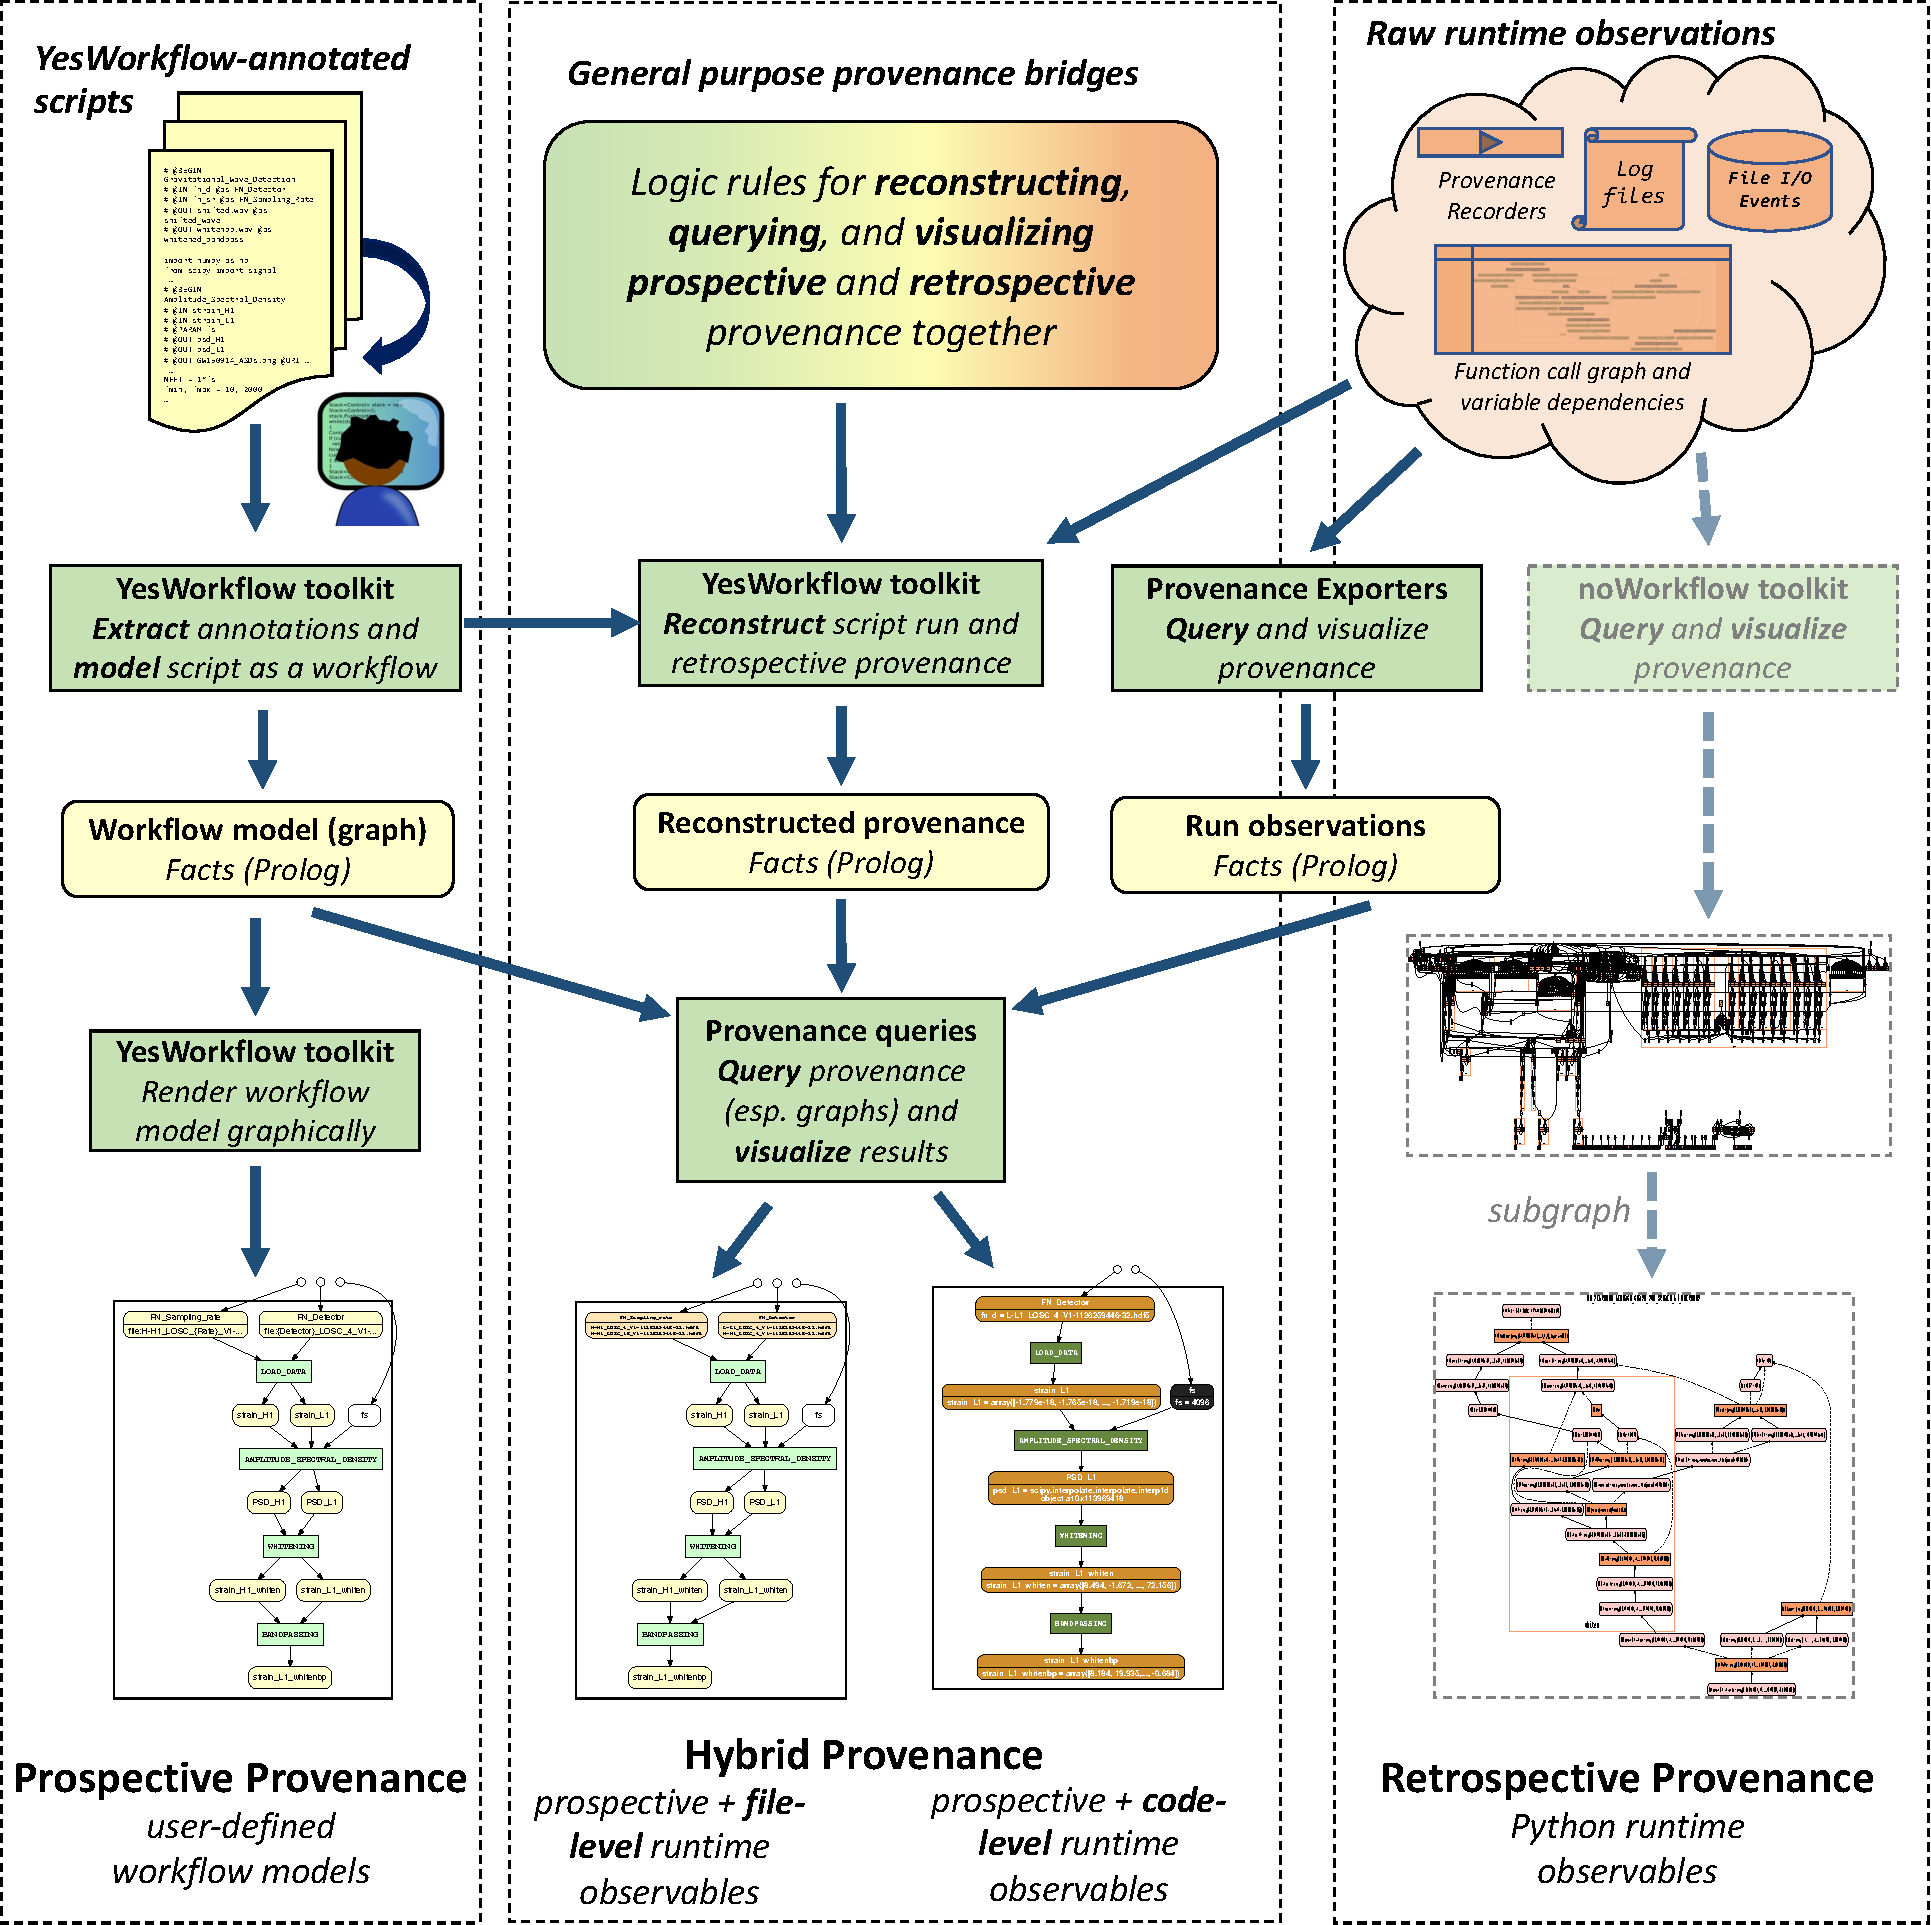
\includegraphics[height=3in, width=\columnwidth]{figures/IDCC-overview-v2-reduced-crop}
  \caption{Provenance Query Architecture}
  \label{fig:prov_query_arch}
\end{figure}

\paragraph{\textit{\bf Prospective provenance tool (YesWorkflow) and retrospective provenance tool (RunManagers)}} 

YW and RunManagers that are used by DataONE provenance team are used for demo. YesWorkflow (YW) is a prospective provenance tool allowing users to easily recover high-level workflow models latent in scripts using simple user-annotations embedded as script comments [ref]. The workflow models declared by users and extracted via the YW toolkit can be augmented and enriched by retrospective provenance observables, yielding different forms of hybrid provenance [ref ...], i.e., whose ``workflow backbone" is given by the user-declared YW model (prospective provenance) and whose execution details are filled in from one or more sources of runtime observables (retrospective provenance), cf. Figure~\ref{fig:yw_tags}.

Figure~\ref{fig:yw_tags} shows a code snippet from a MATLAB script with YW annotations: Here, the @begin and @end tags are used to mark code blocks (i.e., processing steps in the YW model); @in and @out tags are used to define the dataflow between blocks; and the @uri template (which is paired with an @in tag) is used to define a where the data file is located. Note that @uri templates define a metadata pattern via so-called template variables (here: ${start\_year}$, ${end\_year}$, and ${month}$). In this way, the script author can document the folder structure and file-naming conventions used by the script. When the script is run, concrete file- and folder-names are instantiated and can be harvested subsequently by YW to obtain runtime provenance information (even in the absence of a dedicated provenance recorder [ref]). When combining this retrospective provenance information with the YW workflow model, hybrid provenance queries can be answered.

\begin{figure}
  \includegraphics[width=\columnwidth]{figures/YW_annotation_example}
  \caption{An example YW annotation block in the C3C4 script}
  \label{fig:yw_tags}
\end{figure}

RunManagers are DataONE provenance tools for capturing retrospective provenance from MATLAB and R script executions. The DataONE RunManagers
overload and thus intercept file I/O operations to automatically capture runtime observables at the file level. DataONE provides two implementations: the recordr R package and the MATLAB toolbox. The provenance captured during a script execution includes information about the script that was run, the files that were read or written, and details about the execution environment at the time of execution.

The retrospective provenance tool (DataONE RunManagers) support the APIs for R and MATLAB users to capture, search, archive, and share a script run, such as, \texttt{record()}, \texttt{startRecord()}, \texttt{endRecord()}, \texttt{listRuns()}, \texttt{deleteRuns()}, \texttt{viewRun(s)()}, \\ \texttt{traceRuns()} for R, \texttt{plotRuns()} for R and \texttt{publishRun()}. The captured retrospective provenance are populated to a relational provenance database which has these tables for \texttt{execution metadata}, \texttt{file metadata}, \texttt{tag}, \texttt{module dependencies} for MATLAB and \texttt{prov relationships} for R. Furthermore, these relational retrospective can be exported to Prolog facts and YAML formats. On the other hand,  the captured provenance can be packaged and published to the DataONE member node federation network. A DataONE provenance package includes the script itself, input files, generated files that are associated with the run, science metadata file that documents the run and a resource map. 

\section{Example Use Cases} \label{usecases}

In this demo, two real-life scientific examples are used: (1) a workflow for Ocean Health Index (OHI) for Howe Sound, British Columbia [ref]; (2) a workflow for Carbon3/Carbon4 (C3/C4) soil mapping for North America [ref]. The OHIBC Howe Sound workflow runs in a batch mode.

Based on RunManager R provenance database, Figure~\ref{fig:hs_trace_graph} gives us an overview for the OHIBC Howe Sound workflow example. The goal model for Howe Sound is: a region's status is based upon percent of protected area within 1 km inland buffer and percent of protected area within 3 nautical mile offshore buffer, compared to a reference point of 30\% protected area. The data sources used in the OHIBC workflow include: (1) BC-specific WDPA dataset that was created from WDPA global dataset, then rasterize to BC Albers at 500m resolution; (2) BC Parks, Ecological Reserves, and Protected Areas (PEP) data. The OHIBC workflow creates two outputs: one file is for estimate of status by region since 1980 (\texttt{lsp\_status.csv}) and the other file is for estimate of trend by region since 1980 (\texttt{lsp\_trend.csv}). Figure~\ref{fig:hs_trace_graph} also shows the methods used in the OHIBC workflow example and each method name is represented using a script name. For example, the script \texttt{rasterize\_HS\_WDPA\_and\_PEP.R} rasterizes the BC WDPA-MPA shapefile to Howe Sound extents; the script \texttt{lsp\_zonal\_stats.R} calculates the goal model for Howe Sound explained above; and the script combines scores for inland and offshore and writes to output layers (\texttt{estimate\_status\_and\_trend\_by\_year.R} ).

\begin{figure}
  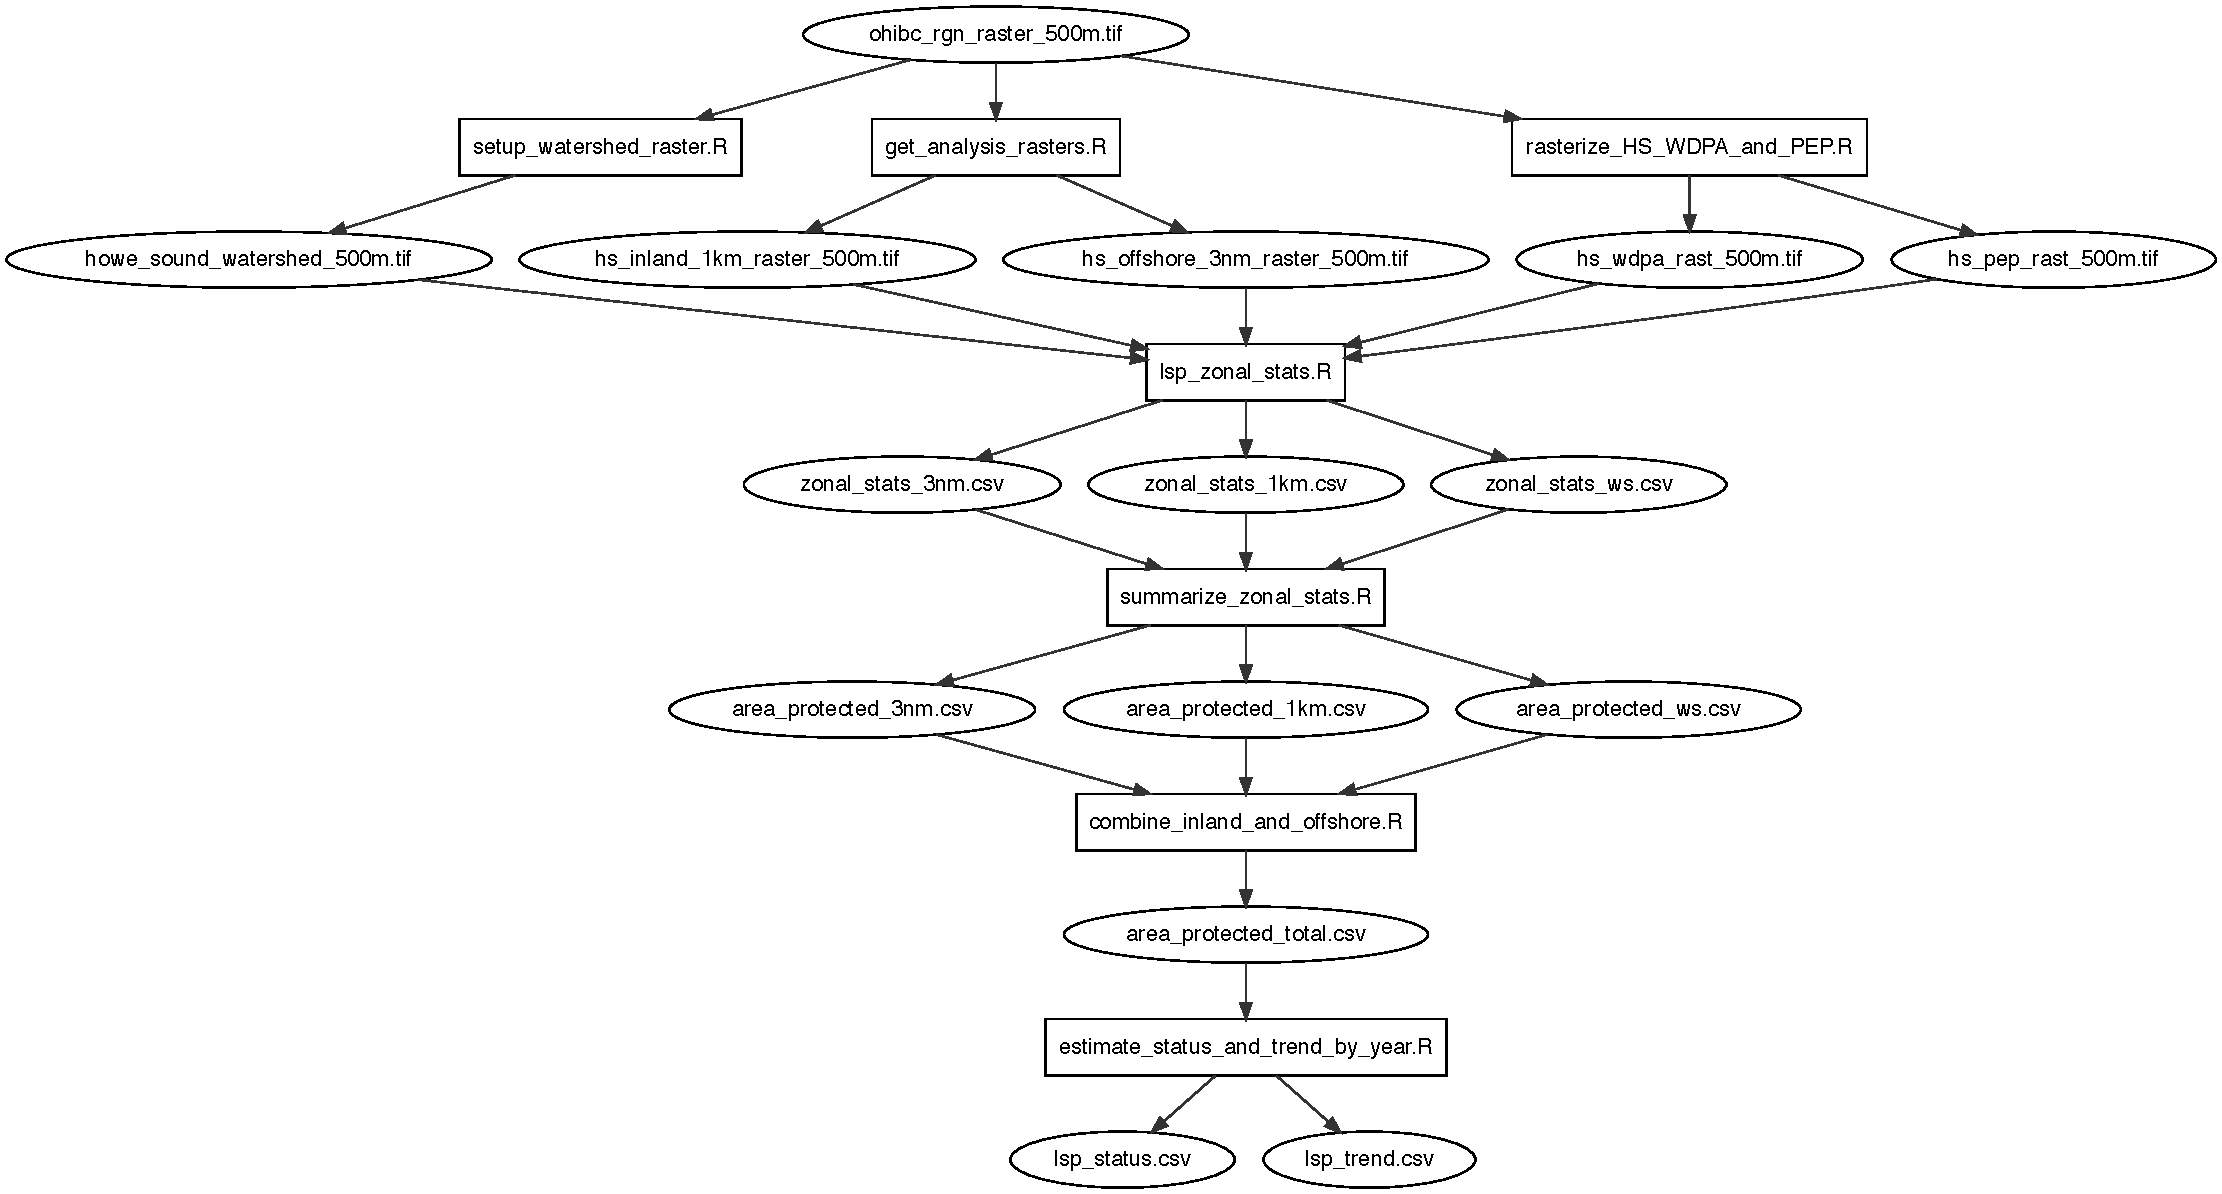
\includegraphics[height=3in, width=\columnwidth]{figures/trace}
  \caption{Complete retrospective provenance graph for the OHI Howe Sound workflow example plotted by the API \texttt{plotRun()} in DataONE RunManager R client}
  \label{fig:hs_trace_graph}
\end{figure}


\begin{figure*}
  \centering
  \subfloat[label1]{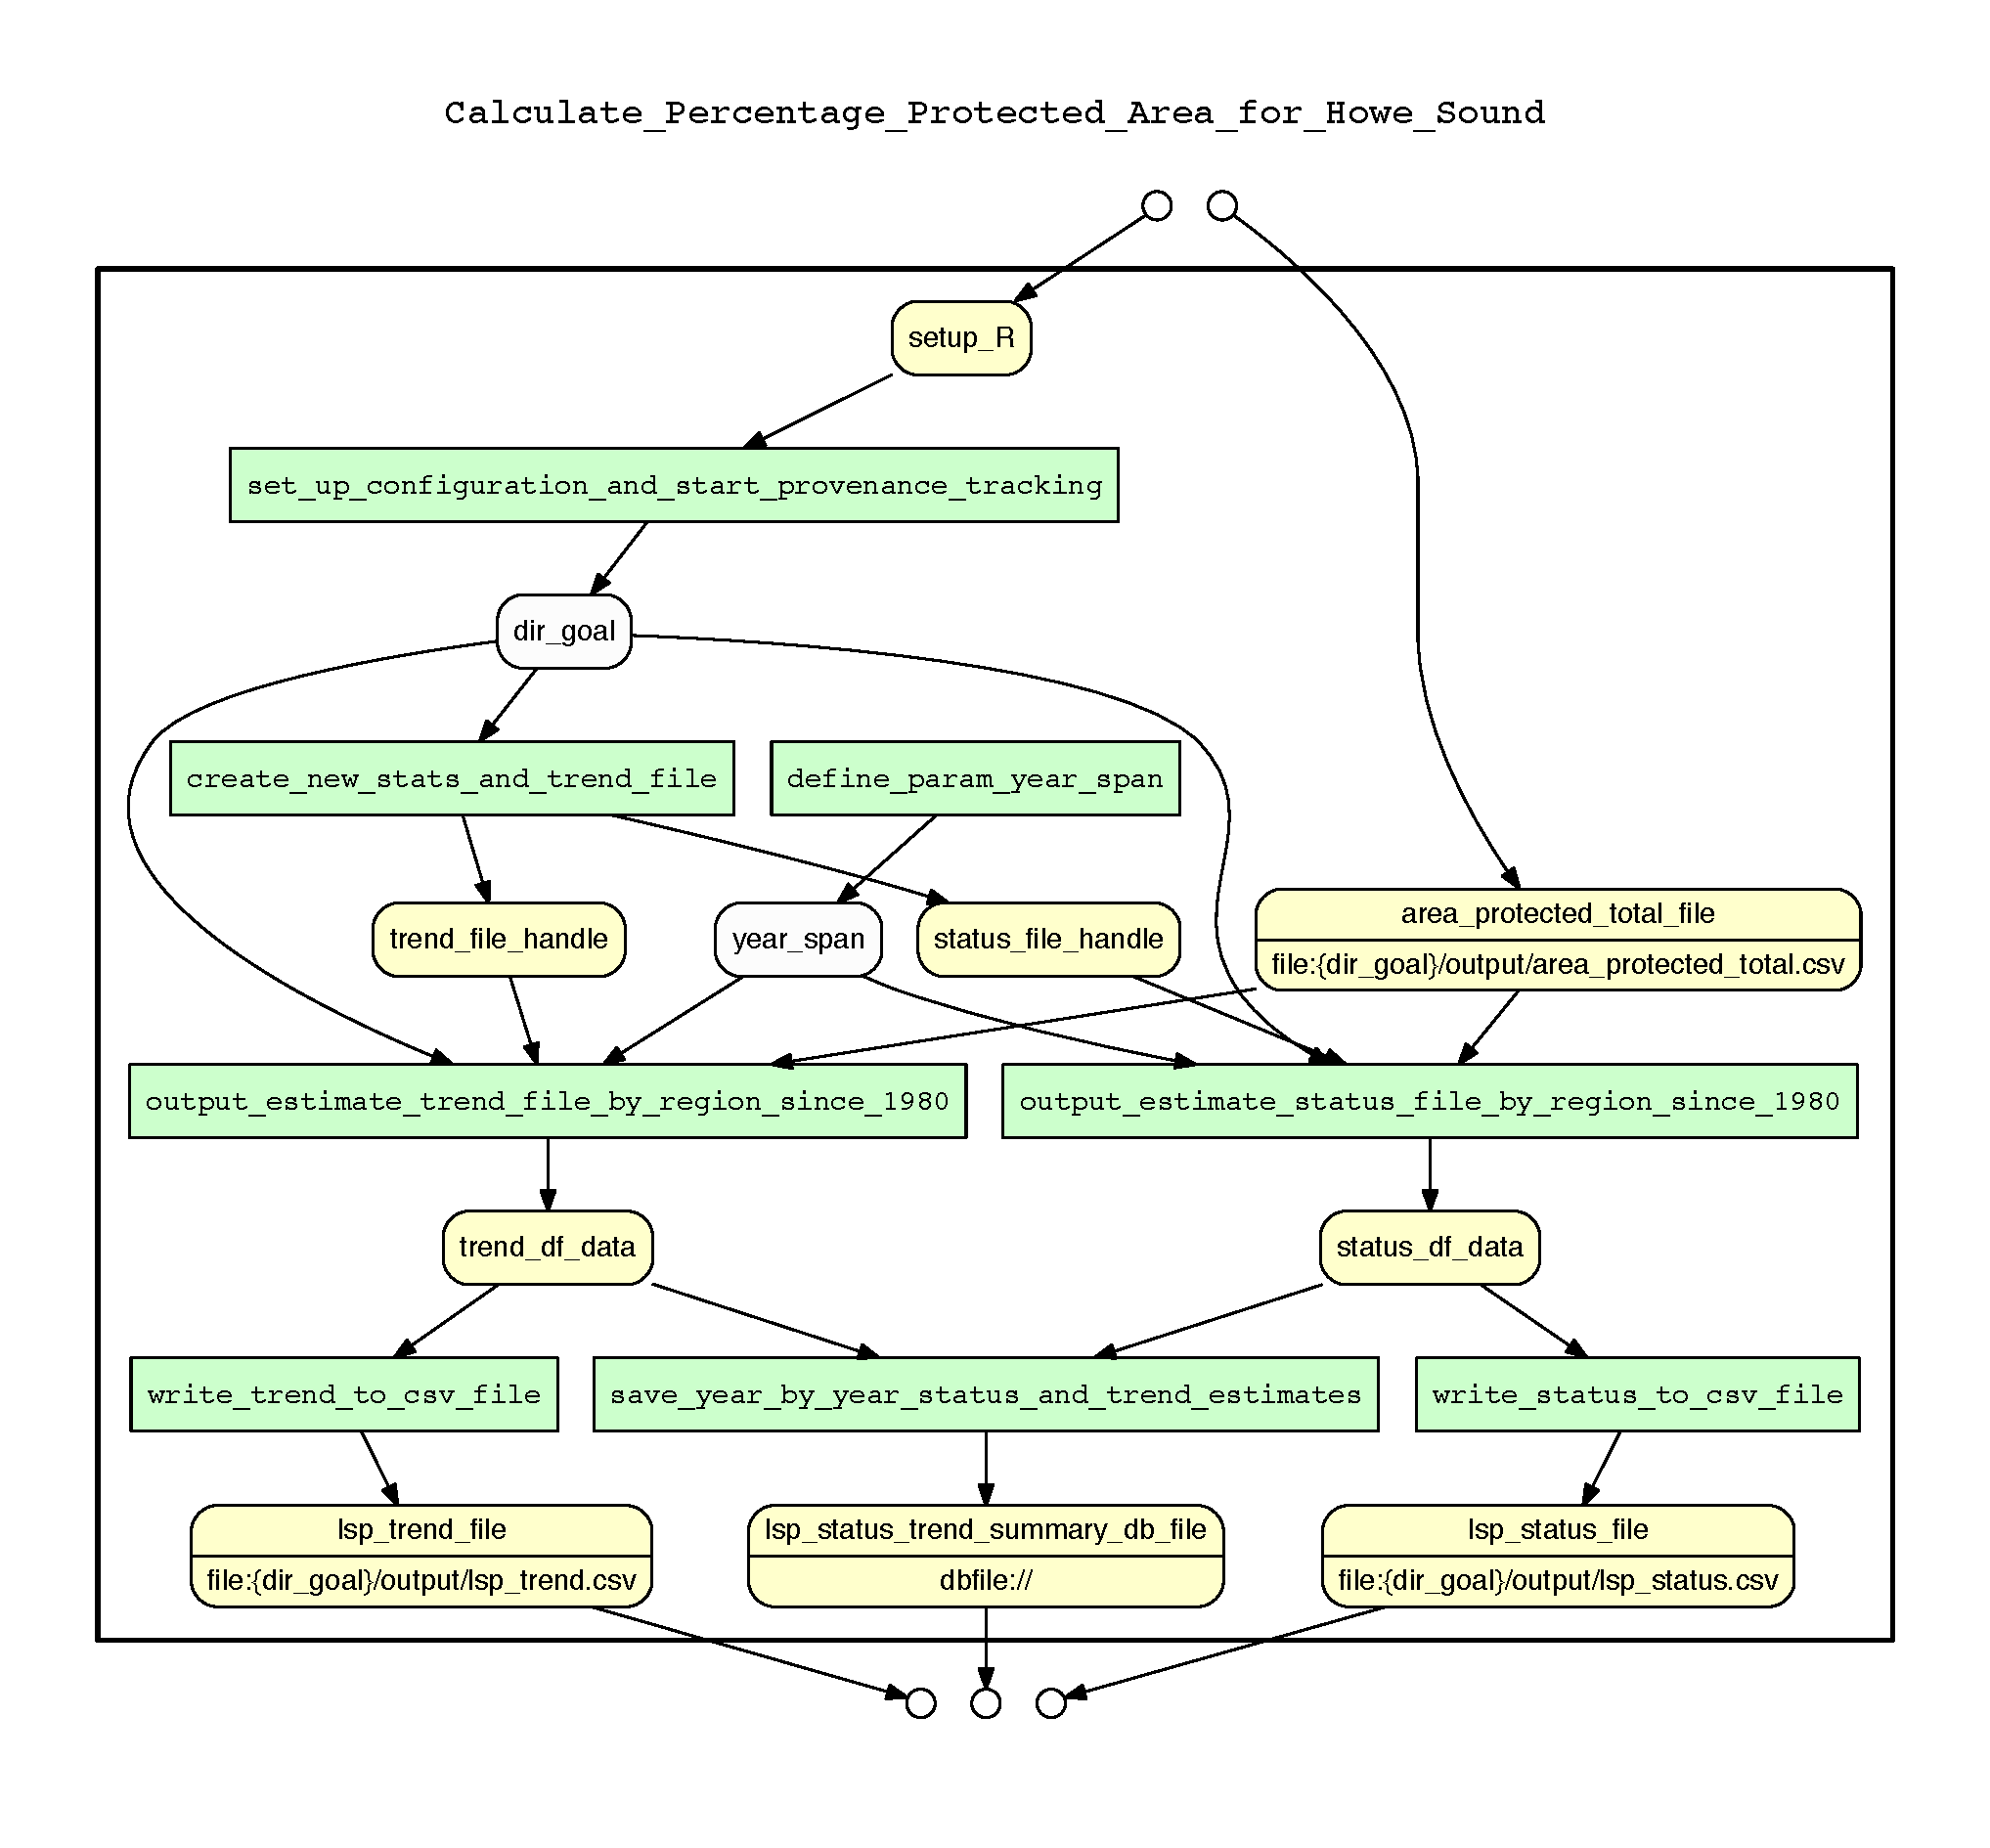
\includegraphics[width=\columnwidth]{figures/OHI_complete_wf_graph_uri}}
  \subfloat[label2]{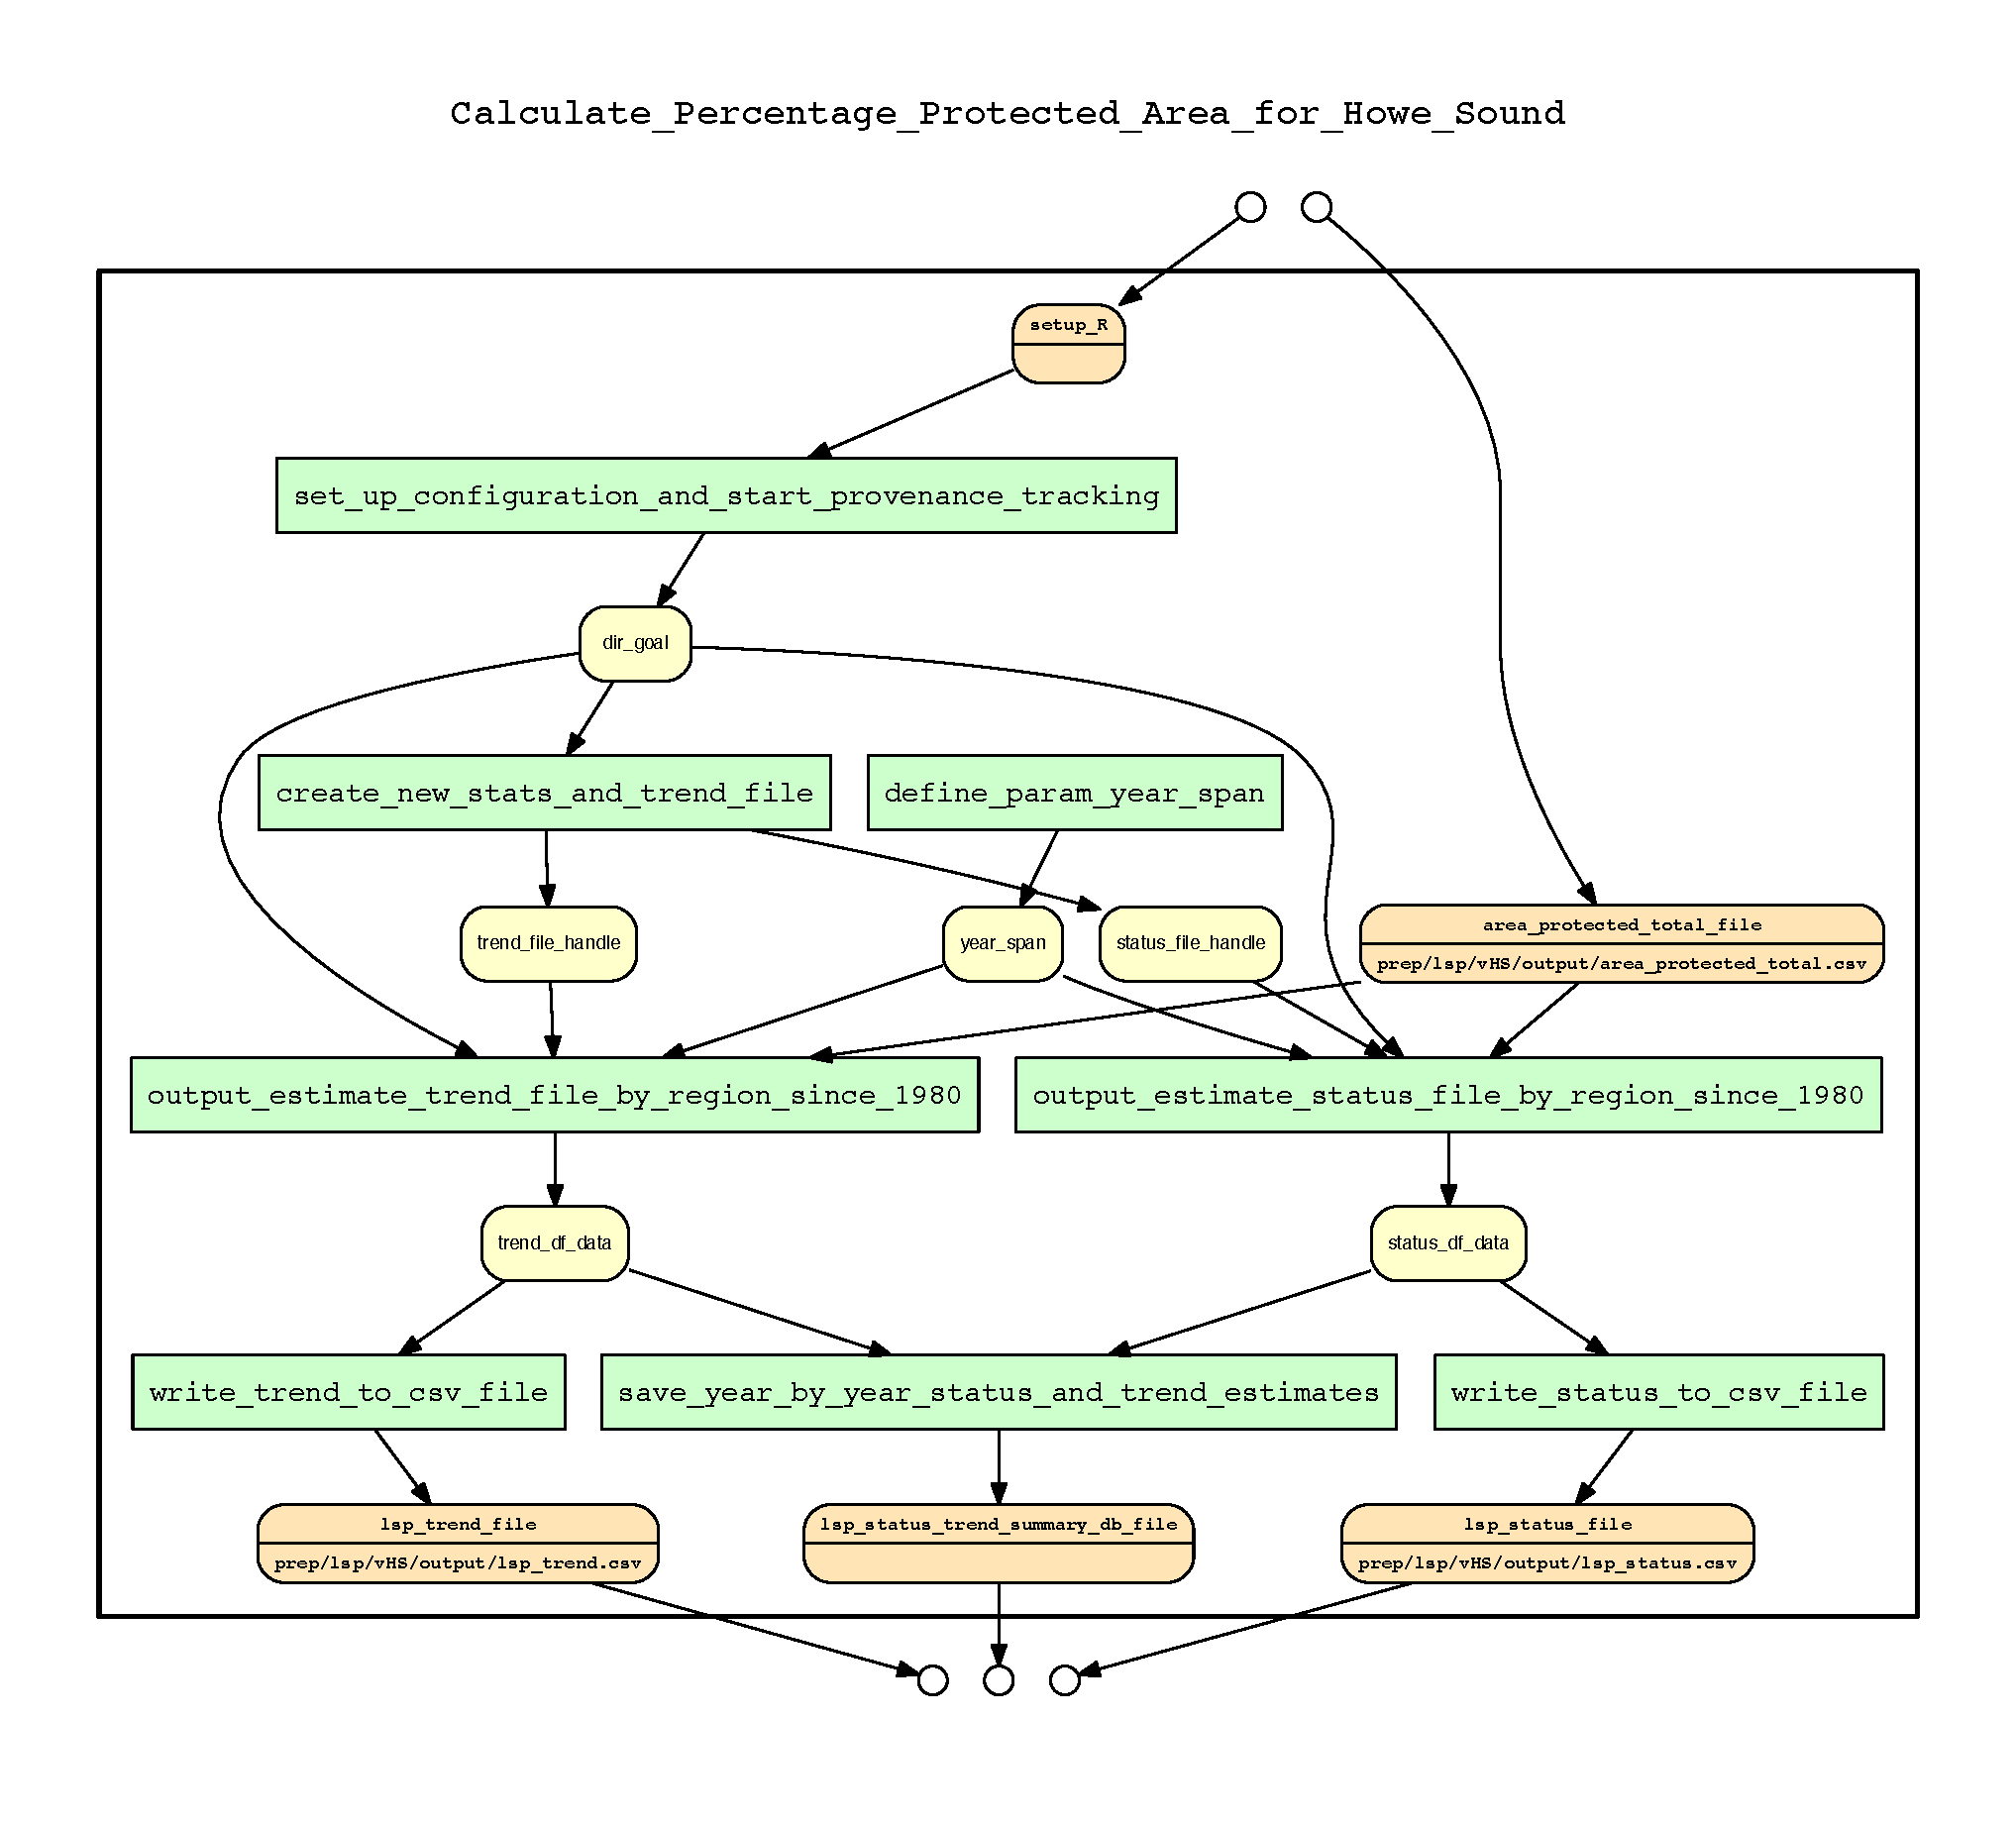
\includegraphics[width=\columnwidth]{figures/OHI_recon_complete_graph_all_observables}}
  \caption{Complete YW prospective and hybrid provenance graphs for the OHIBC Howe Sound example. The diagram shows the script \texttt{estimate\_status\_and\_trend\_by\_year.R} that calculates the ``lasting special places�sub goal" of the Ocean Health Index for Howe Sound, British Columbia that is based on the percentage of protected area within 3km of shore and 1km buffer zone inland, and how that has changed over time. The green box represents a computation step and a round yellow square box represents a data element declared in the script via YW tags.}
  \label{fig:hs_yw}
\end{figure*}


To demonstrate the provenance data dependency analysis, we have developed SQL queries as well as rule-based queries (implemented in Prolog) against various provenance facts. A graph is used to represent the query results. For example: What outputs does the workflow (script) have? Advanced provenance queries can take the form of regular path queries (RPQs), tree-structure queries, or graph queries and show the data lineage hidden in the provenance information. For example: (1) What are the ancestors or descendants of a given output in a prospective provenance graph? (2) What are the ancestors or descendants of a given output in a retrospective- or hybrid- provenance graph? (3) Which possible execution (i.e., dataflow) paths satisfy a given regular path expression? In this demo, we show each of these queries in action. The queries can be found at [ref1, ref2].

The first category provenance query is \texttt{prospective provenance queries} that refer to workflow steps and data names declared via YW annotations. A YW prospective provenance query can tell us if an output depends a particular input or if an output depends on all of inputs. Therefore, YW prospective provenance can add finer workflow model information for each script in order to share the relevant computational steps and data elements with others. For example, the script \texttt{estimate\_status\_and\_trend\_by\_year.R} is used as an example (see Figure~\ref{fig:hs_yw}).  The green box represents relevant computational steps, the yellow round box represents data elements (also called data flow) and the white round box represents parameters that are not consumed by computational steps. Hence, the prospective provenance added by YW is valuable for script-based scientific workflow provenance.

The second category provenance query is \texttt{hybrid provenance query}, that is querying YW*DataONE RunManager retrospective provenance. YW*DataONE RunManager hybrid provenance queries refer to YW model and runtime file-level retrospective provenance harvested by RunManager. In a hybrid provenance graph, the ``workflow backbone" is given by the user-declared YW model (prospective provenance) and the execution details are filled in from one or more sources of runtime observables (retrospective provenance). Figure~\ref{fig:hs_yw} shows a hybrid provenance graph for the last script in the OHIBC example \texttt{estimate\_status\_and\_trend\_by\_year.R}. We can see that the yellow round box changes to orange round box and the file path pattern embedded is expanded with runtime relative file paths. This graph can tell us the runtime input files and output files. We have another example for Carbon3/Carbon 4 in which there are twelve files matched the YW URI template. Then the URI template is expanded to twelve files in the orange box so that a user can know the actual used file information.

%\begin{figure}
%  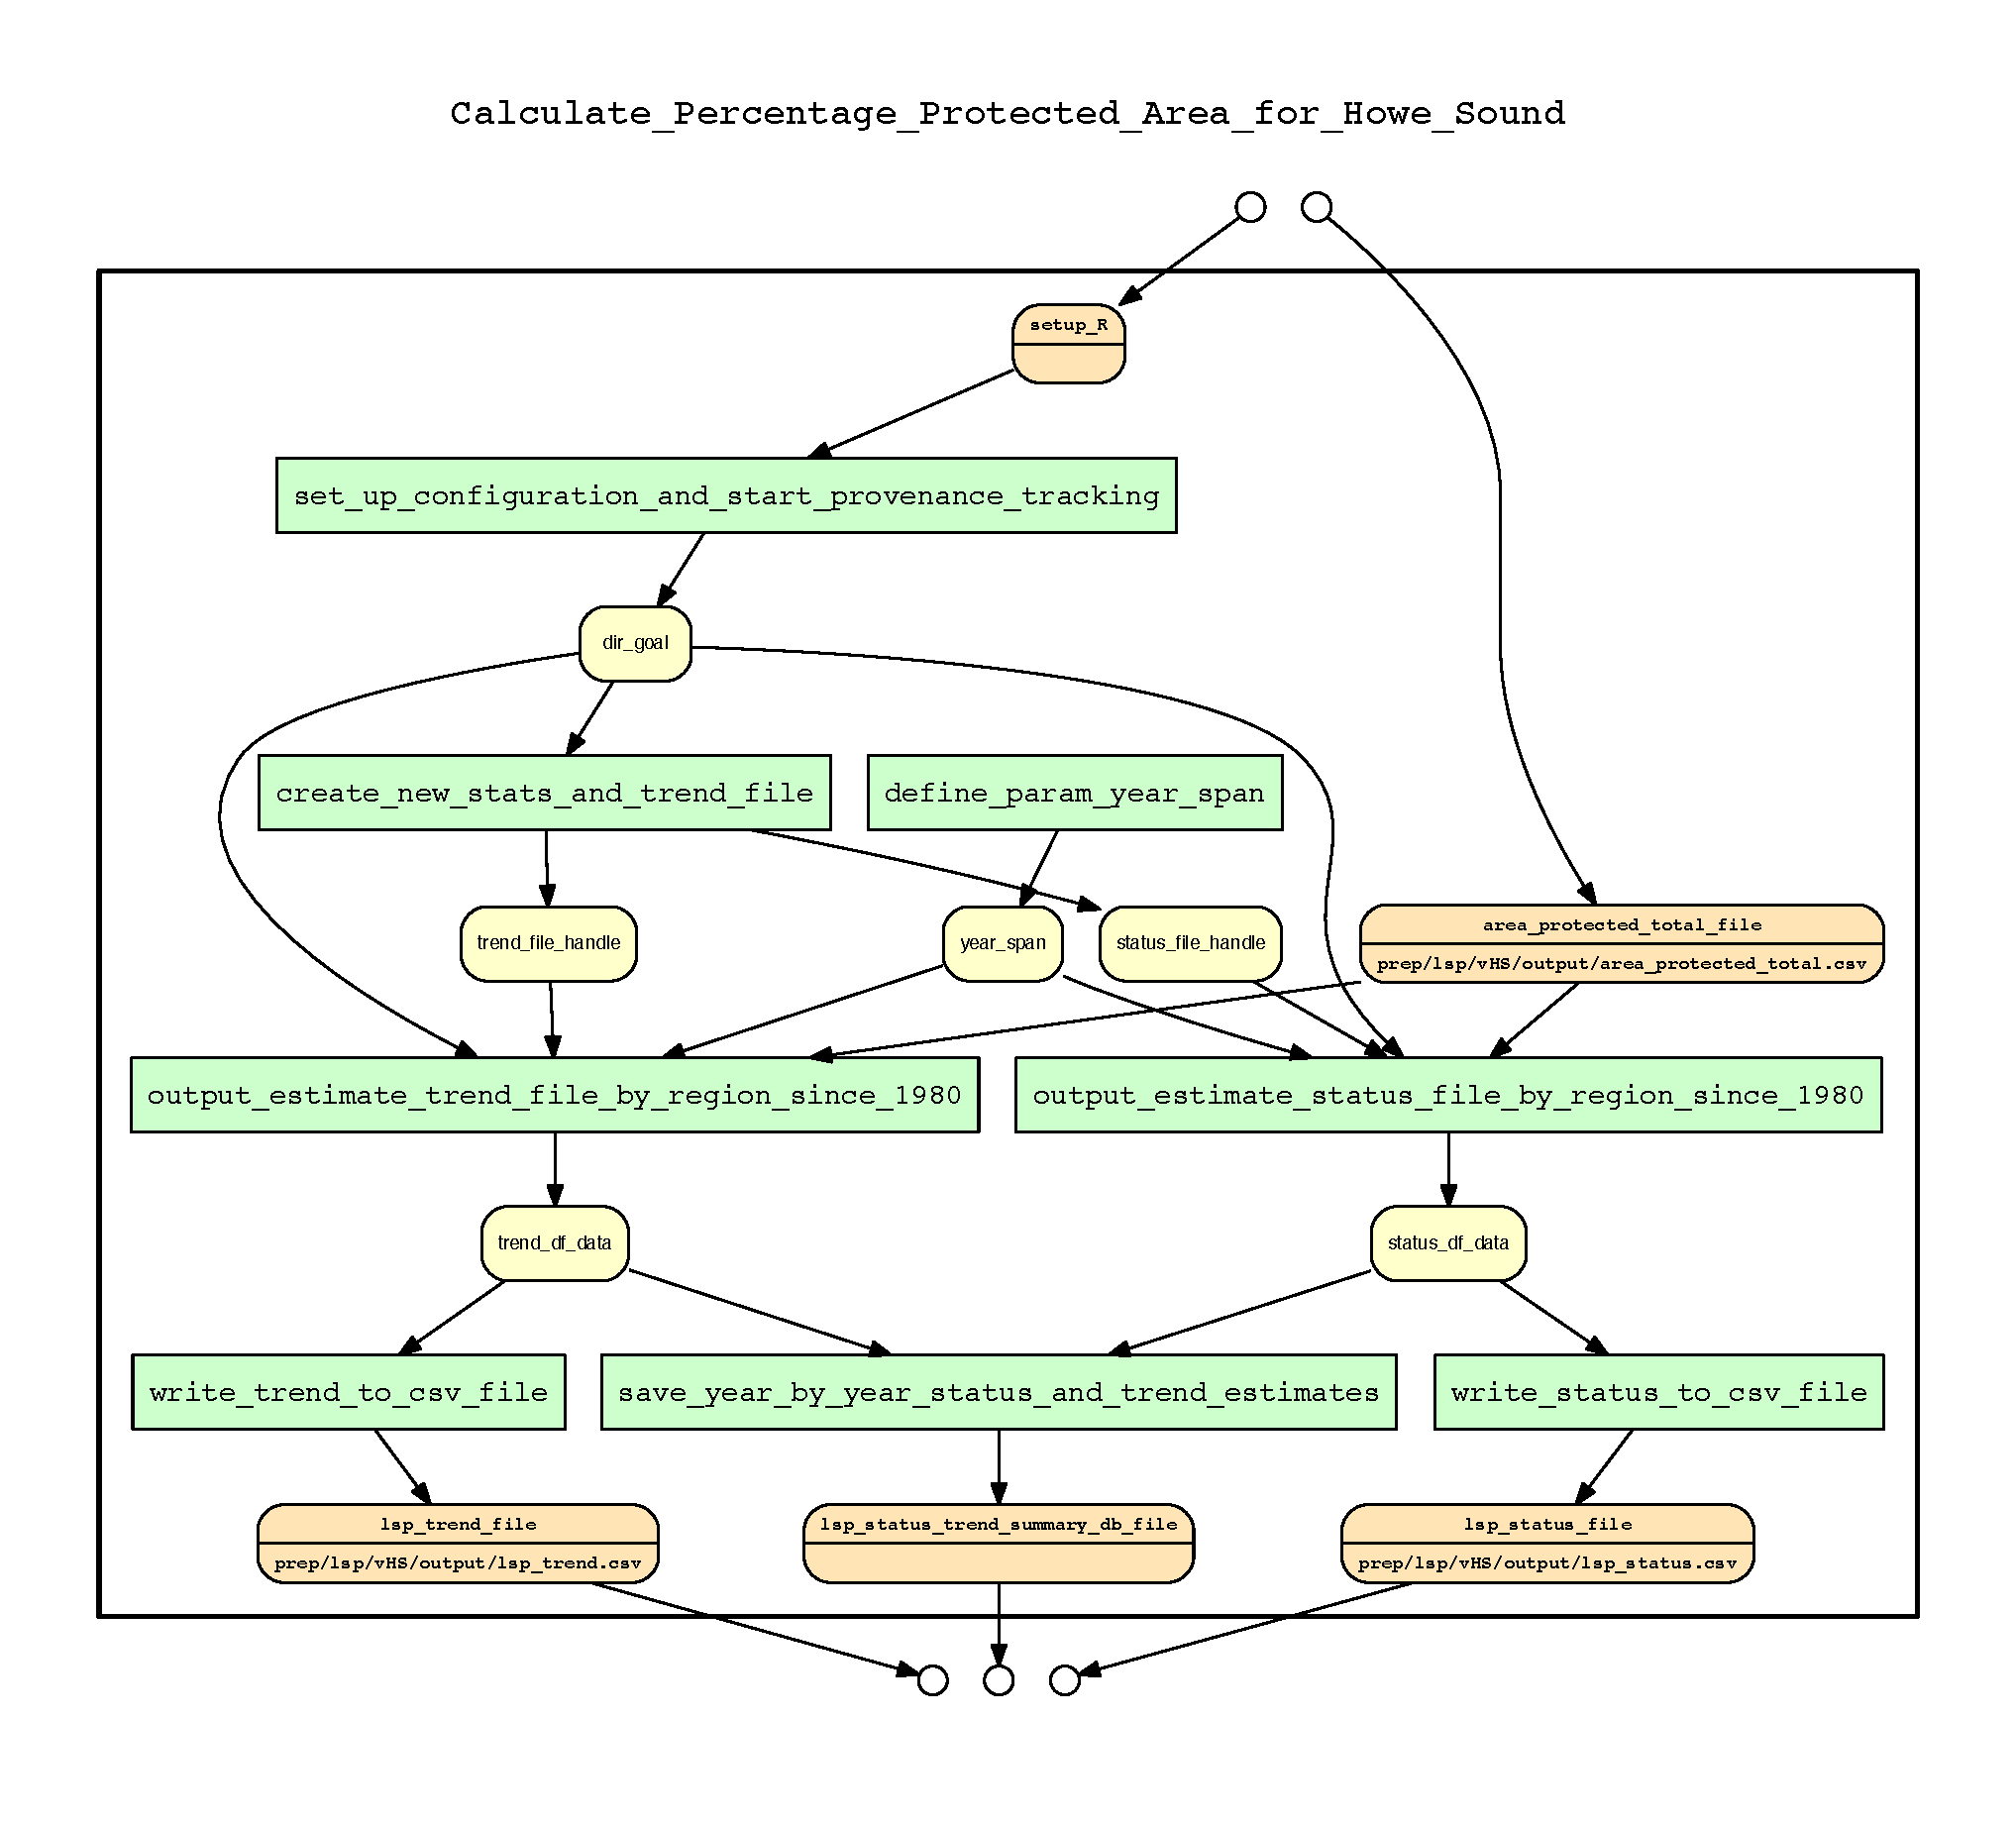
\includegraphics[width=\columnwidth]{figures/OHI_recon_complete_graph_all_observables}
%  \caption{Complete reconstructed hybrid provenance graph for the OHIBC Howe Sound example using YW and DataONE RunManager R client. In the diagram, the runtime file-level observables are augumented with YW prospective graph.}
%  \label{fig:hs_hybrid}
%\end{figure}

The third category provenance query is \texttt{multi-run provenance query}, that is querying DataONE RunManager retrospective provenance. RunManager retrospective provenance queries refer to the runtime retrospective provenance obtained from executing multiple scripts, using RunManager. Since the scripts in a project are usually logically connected through sharing some of their inputs and outputs, the corresponding provenance traces are also connected through shared data products. One example is pictured in Figure~\ref{fig:hs_trace_graph} for the OHIBC workflow example. Besides this valuable overview graph, we provide other formats of multi-run provenance graphs for scientific workflow management: multi-run graph based on file path and multi-run graph based on hash code(see Figure~\ref{fig:c3c4v2_filepath}). 

The second example script (in MATLAB) produces Carbon 3/Carbon 4 (C3/C4) soil maps for North America using average rain and air temperature monthly data from year 2000 to 2010. In order to simulate real-life workflow, we create a version 2 C3/C4 example by splitting one script to three phases: preparing step, examining pixels for grass and generating final results. After the preparing step, a user can run the second script \texttt{examine pixels for grass} for multiple times with different parameters in order to find a proper solution, then writes to the output files. The generated graph recorded a set of runs that consist of the three scripts, five runs and the second script was run with two different parameter values (i.e., 2.5 and 5) twice. Figure~\ref{fig:c3c4v2_filepath} depicts two views of multi-run graphs. By comparing these two figures, we can understand that the second script which was run twice produces two versions of files but write to the same file locations.

\begin{figure*}
  \centering
  \subfloat[label 1]{{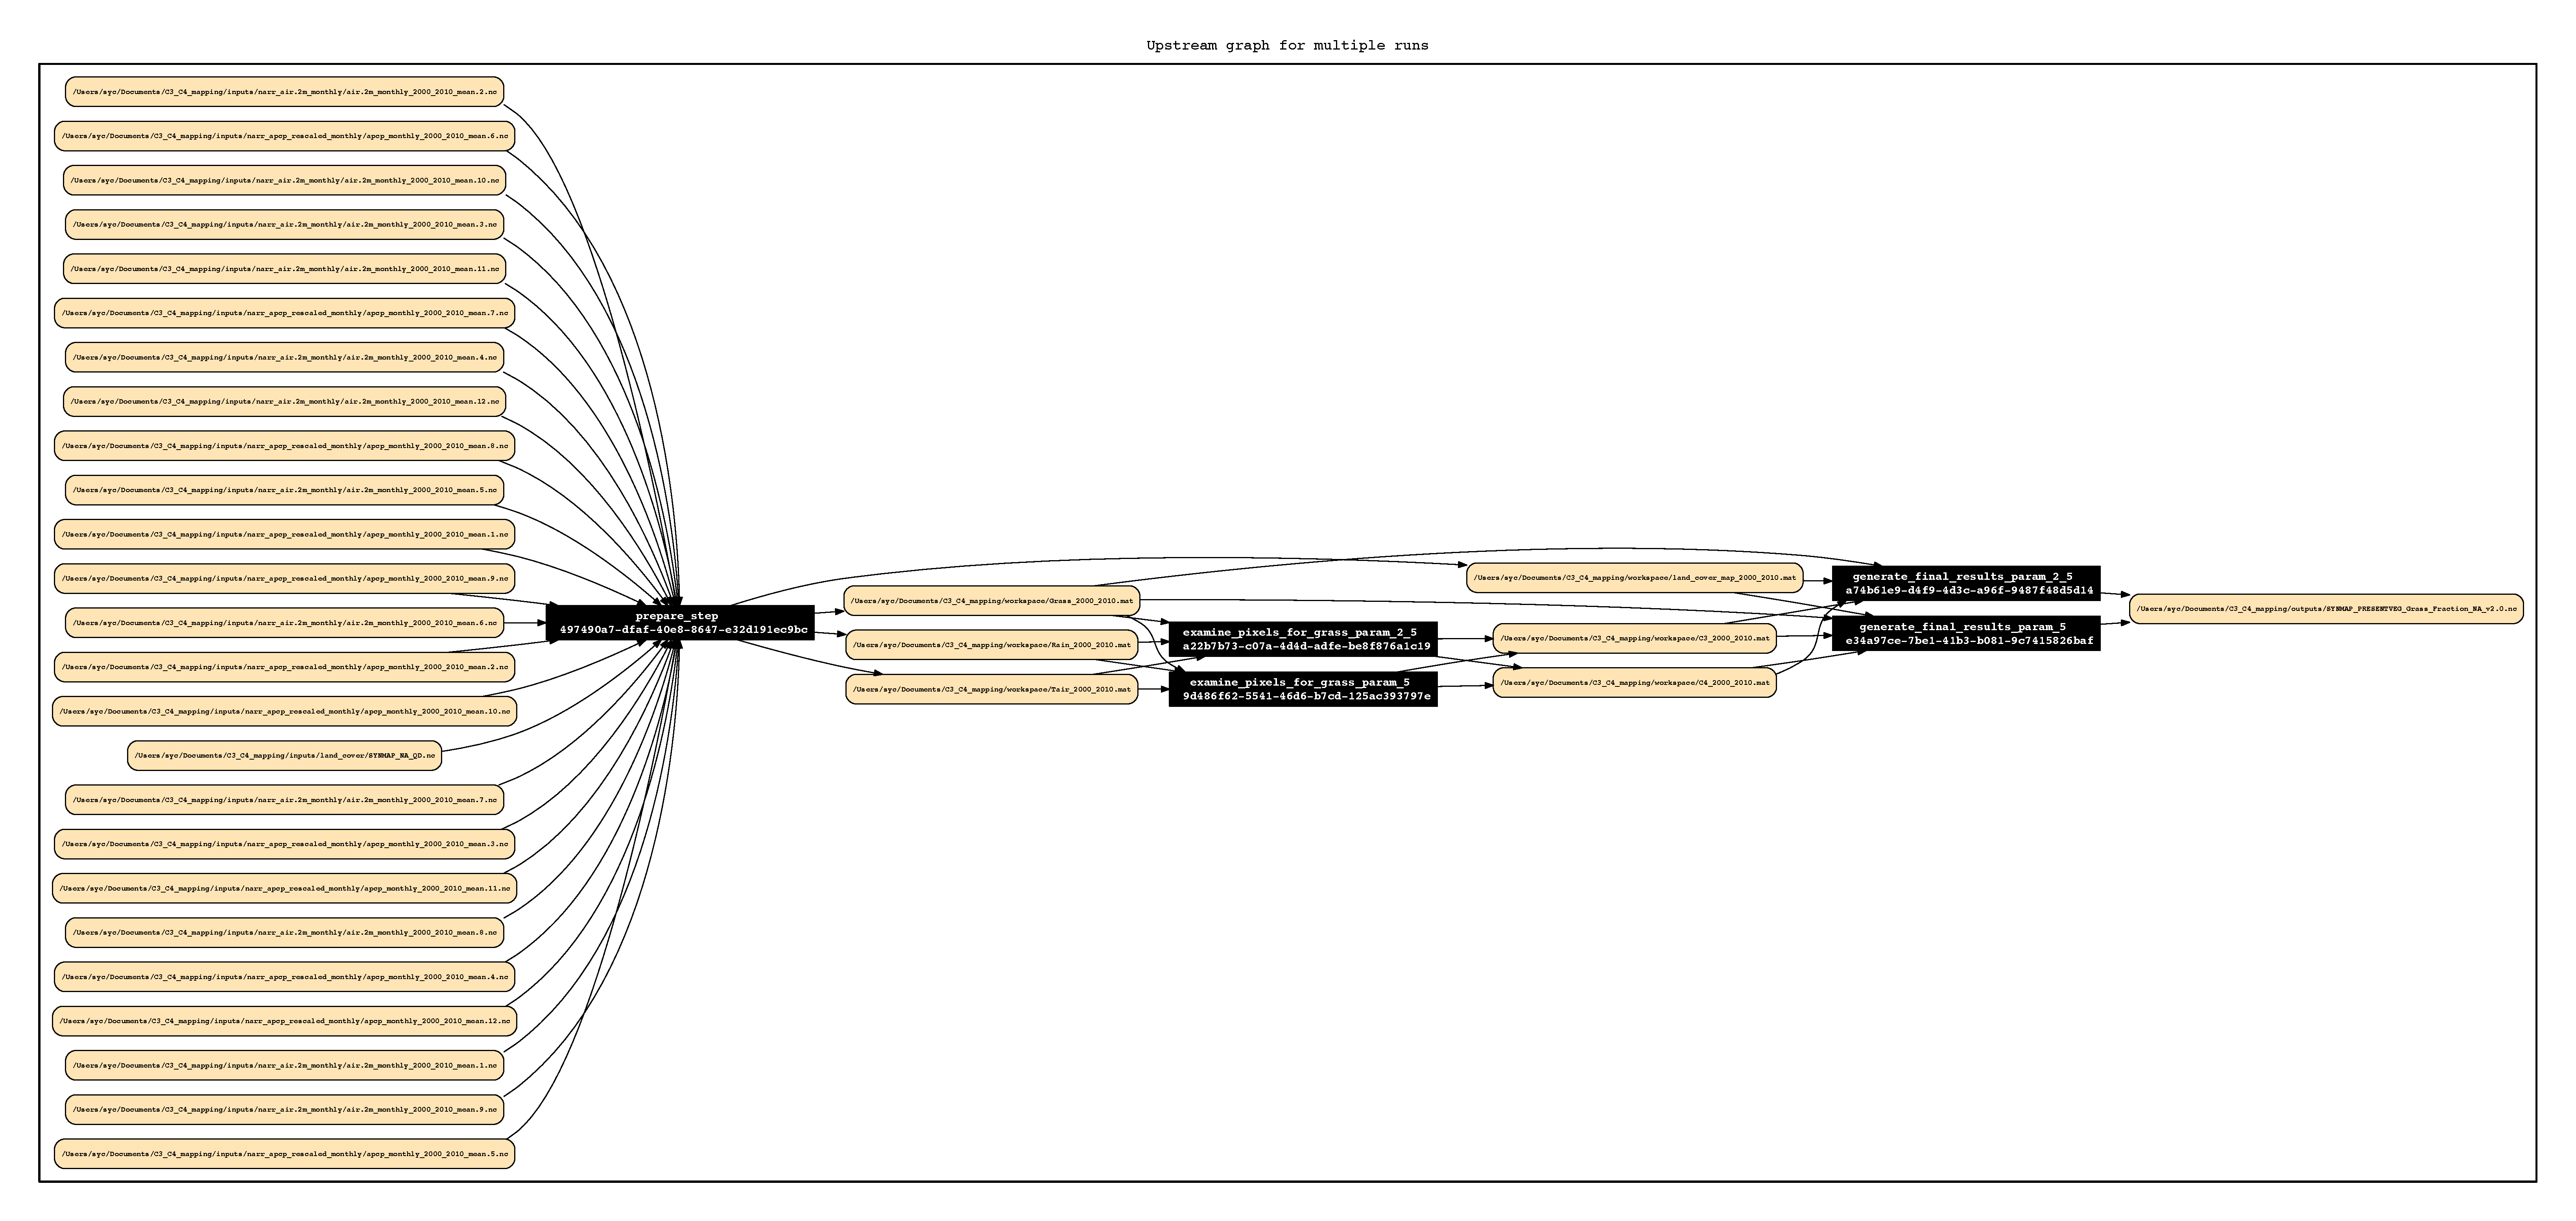
\includegraphics[height=4in, width=\columnwidth]{figures/C3C4v2_upstream_of_Grass_filePath} }}
   \subfloat[label 2]{{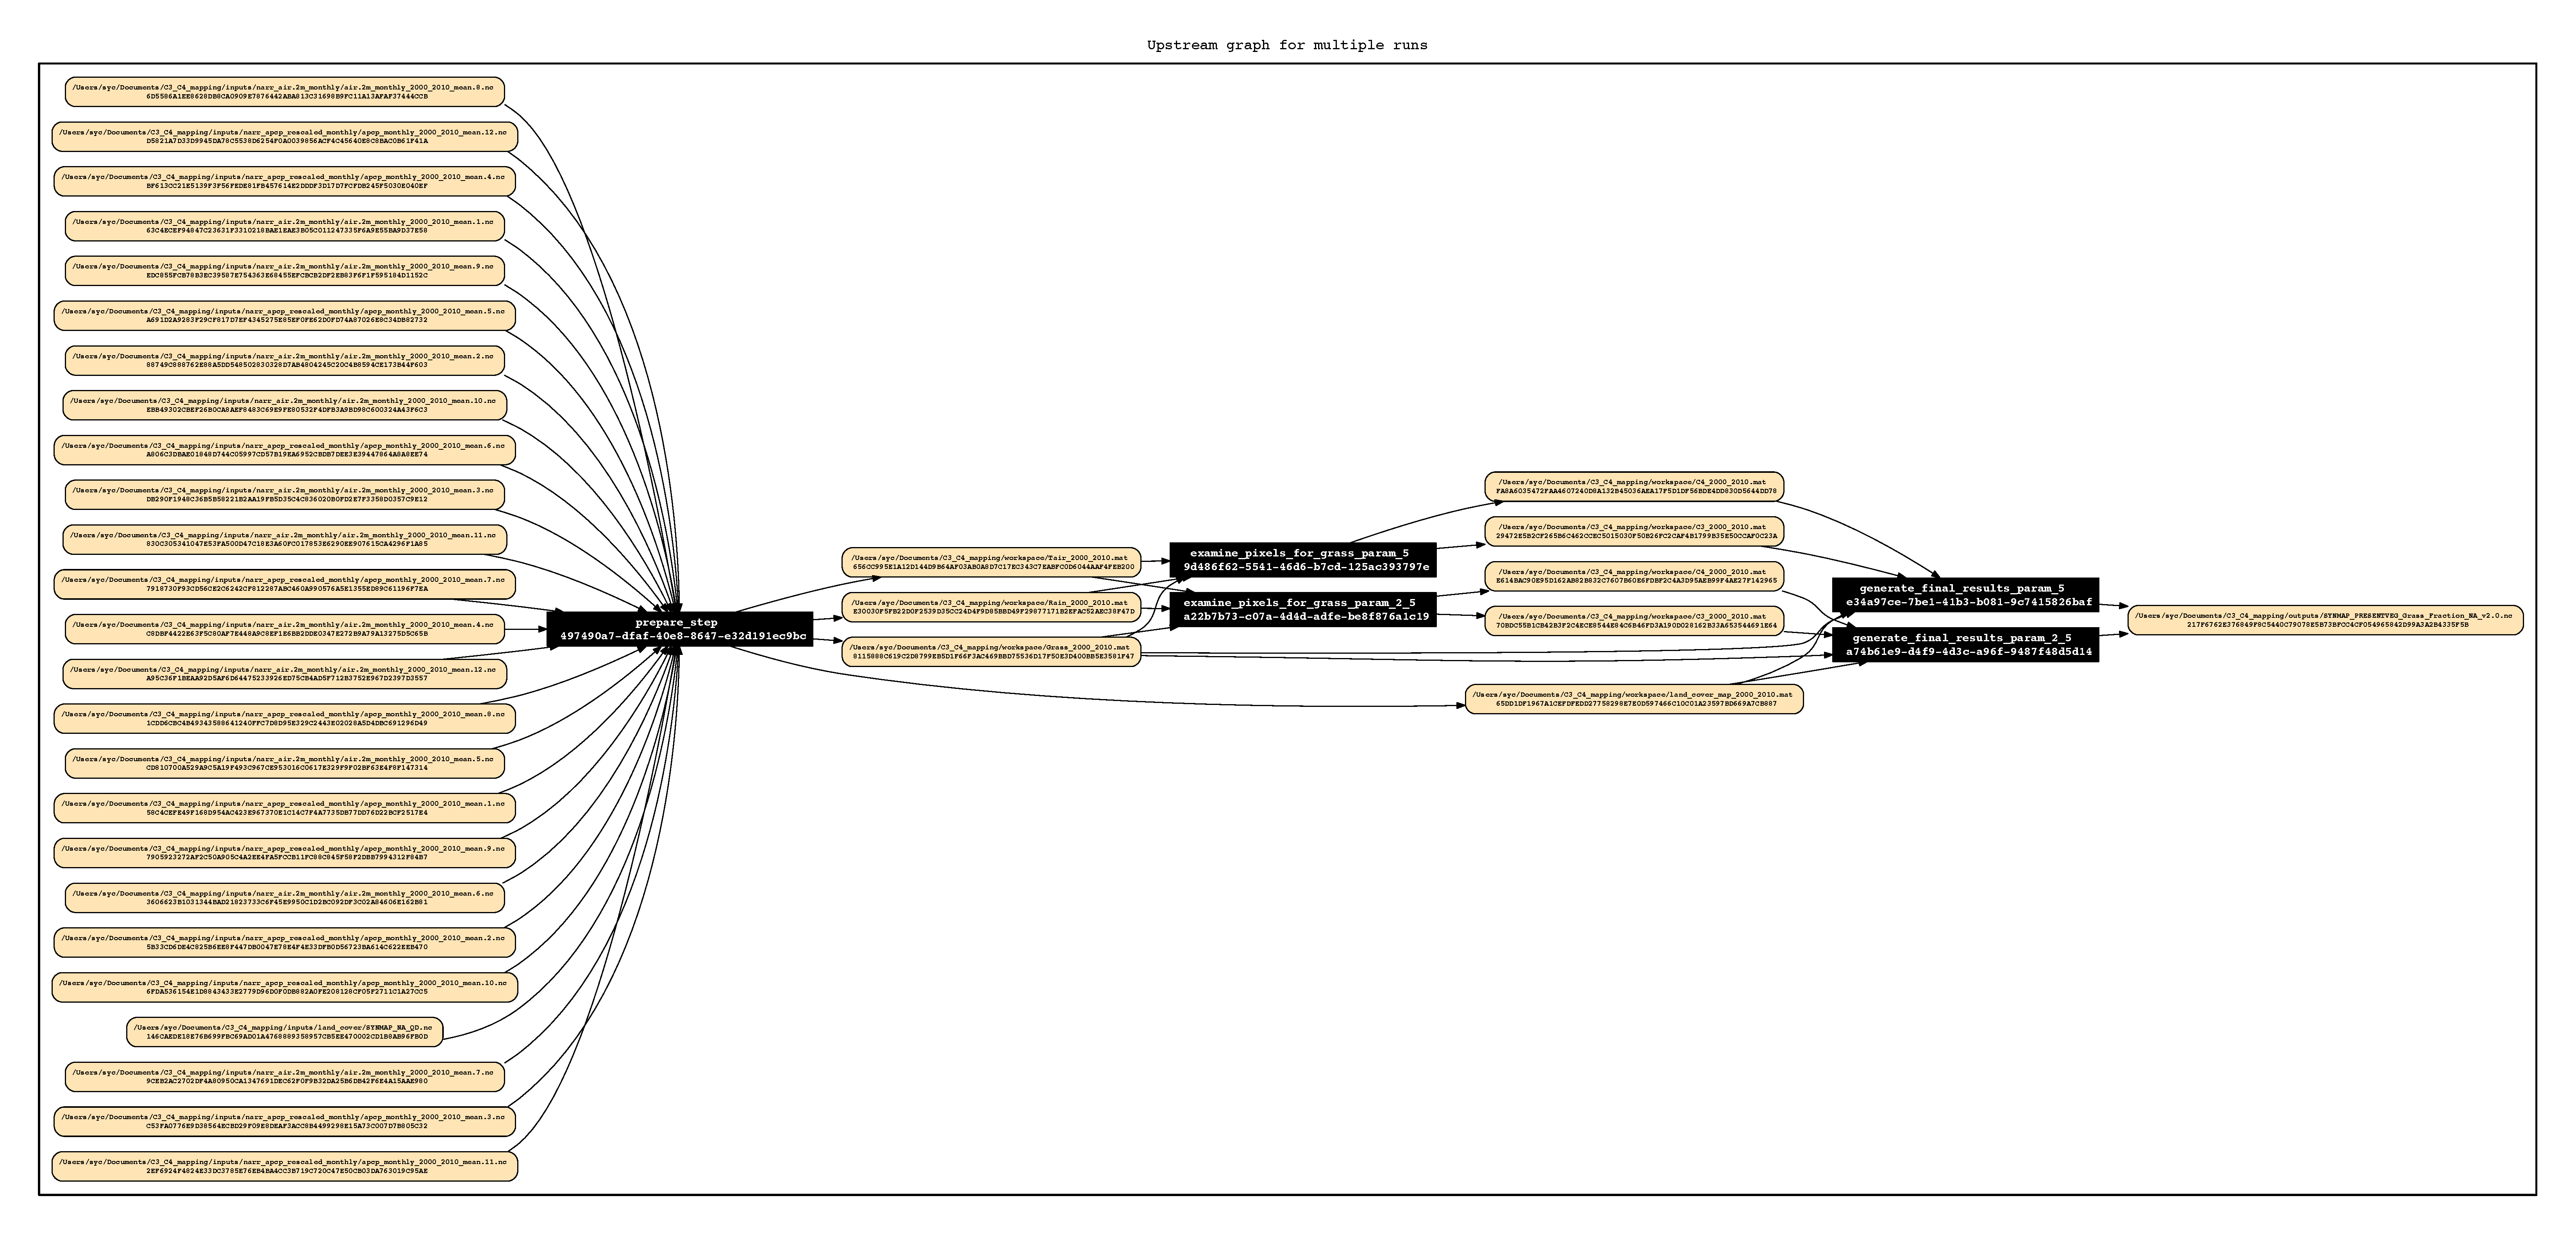
\includegraphics[height=4in, width=\columnwidth]{figures/C3C4v2_upstream_of_Grass_sha256} }}
   
  \caption{Upstream retrospective provenance subgraph (longitudinal view) that is relevant to one output ``\texttt{SYNMAP\_PRESENTVEG\_Grass\_Fraction\_NA\_v2.0.nc}" for C3C4 version 2 example. The presented graph recorded a set of runs that consist of three scripts, five runs and the second script was run with two different parameter values (i.e., 2.5 and 5) twice. The example script set is called C3C4 example version 2. In the diagram, an orange yellow box represents a data file and a black box represents an execution (a run). }
  \label{fig:c3c4v2_filepath}
\end{figure*}

\paragraph{\textit{\bf Reproducibility}}
DataONE allows to make experiments reproducible by providing two capabilities. First, as we have demonstrated above, DataONE RunManagers are able to capture both prospective and retrospective provenance (following the ProvONE model) by keeping tracking of the complete user-defined workflows implicit in a workflow script as well as the full history of the data file produced and consumed during each execution. Second, DataONE data repository allows users to package workflow results (implemented in any programming languages such as Python, R, MATLAB, SAS, ... ) in a structured DataONE data package and publish to a member node inside a DataONE federation network so that the workflow results (including 2D graphs, 3D graphs, scripts, data, provenance relationship, science metadata describing the experimental methods, authors, geographical coverage,  time coverage provided by data providers, ...) can be displayed on DataONE data repository and be shared or linked with other scientific experiments in a larger scale. It is different from providing reproducibility based on IPython notebook [ref] or a virtual machine, such as a Docker or a VM. Compared to myExperiment [ref], DataONE package contains provenance information (\texttt{prov:used}, \texttt{prov:wasGeneratedBy}, or \texttt{prov:wasDerivedFrom}) to describe the relationships between digital objects and datapackages for reproducibility, although both myExperiment and DataONE use package to encapsulate digital objects such as input data, final results and provenance. 

\section{Conclusions}  \label{conclusions}

Provenance is a useful component of the software development cycle, either to benefit researcher themselves or documenting and sharing code for use by future investigators. For the researcher, the quality of data produced by script runs can be assessed by identifying source data and verifying their quality. 

Many provenance tools have been developed to capture, store, query and visualize the provenance produced by scripts and runs of scripts. But there is not enough investigation on what kind of provenance queries can be answered from the provenance information at prospective and retrospective provenance levels. Our research on prospective, hybrid and retrospective provenance queries allow researchers to use simple queries and a subset of advanced queries to query across YW model and various retrospective provenance sources to produce interesting provenance artifacts. 
      
With our provenance query demo, we showcase our prospective, retrospective and hybrid query capabilities. We demonstrated that provenance queries across heterogeneous provenance sources can yield a more complete and comprehensible picture of data provenance. We also think provenance describing datasets can facilitate data discovery for others. 


\bibliographystyle{ACM-Reference-Format}
\bibliography{sigproc} 

\end{document}
